% Copyright 2019 Clara Eleonore Pavillet

% Author: Clara Eleonore Pavillet
% Description: This is an unofficial Oxford University Beamer Template I made from scratch. Feel free to use it, modify it, share it.
% Version: 1.0

% \documentclass[notes]{beamer}
% \documentclass[notes=only]{beamer}   % only notes
\documentclass{beamer}
% Load Packages
\usepackage[utf8]{inputenc}
\usepackage{xcolor}
\usepackage{tikz}
\usetikzlibrary{positioning,calc}
\usepackage{graphicx}
\usepackage{hyperref}
\usepackage{amsmath}
\usepackage{listings}
\usepackage{fontawesome}

% Define Commands
\newcommand*{\ClipSep}{0.06cm} %To adjust footer logo
\newcommand{\E}{\mathrm{e}\,} %\def\I{e} % used to defined e for exp(x), see later what it should be
\newcommand{\ud}{\mathrm{d}}
\lstset{numbers=left, numberstyle=\tiny, stepnumber=1,firstnumber=1,breaklines=true,
    numbersep=5pt,language=Python,
    stringstyle=\ttfamily,
    basicstyle=\footnotesize, 
    showstringspaces=false
}

\usetheme{oxonian}

\title{Notes on the development of scale-free network models}
\titlegraphic{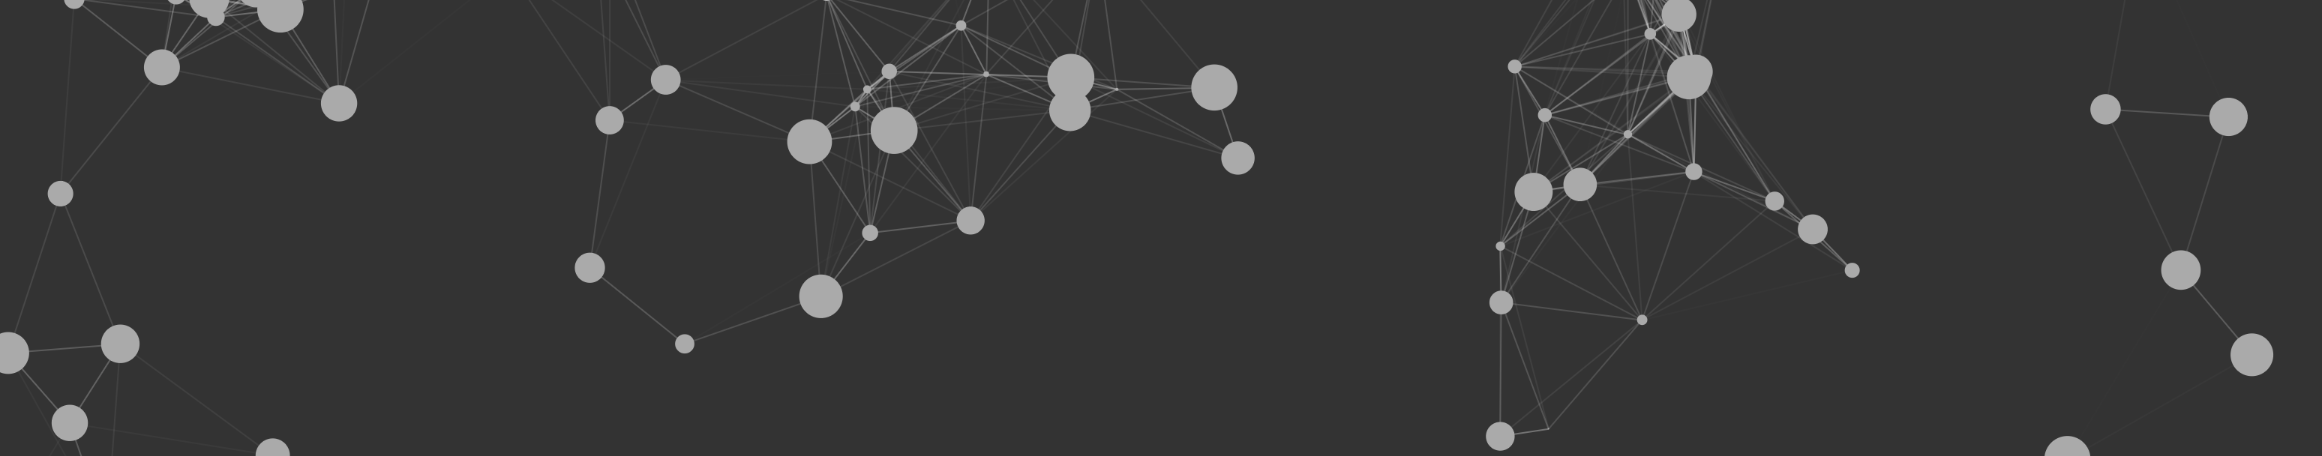
\includegraphics[width=\textwidth]{Theme/Logos/networks-title-img.png}}
\author{Matthew Turner}
\institute{UC Merced, Kello lab meeting}
\date{\today}

\begin{document}

{\setbeamertemplate{footline}{} 
\frame{\titlepage}}

% \section*{Outline}\begin{frame}{Outline}\tableofcontents\end{frame}


\section{Introduction: a perfect scientific storm}
\begin{frame}[plain]
  \vfill
  \centering
  \begin{beamercolorbox}[sep=8pt,center,shadow=true,rounded=true]{title}
    \usebeamerfont{title}\insertsectionhead\par%
    \color{oxfordblue}\noindent\rule{10cm}{1pt} \\[1em]
    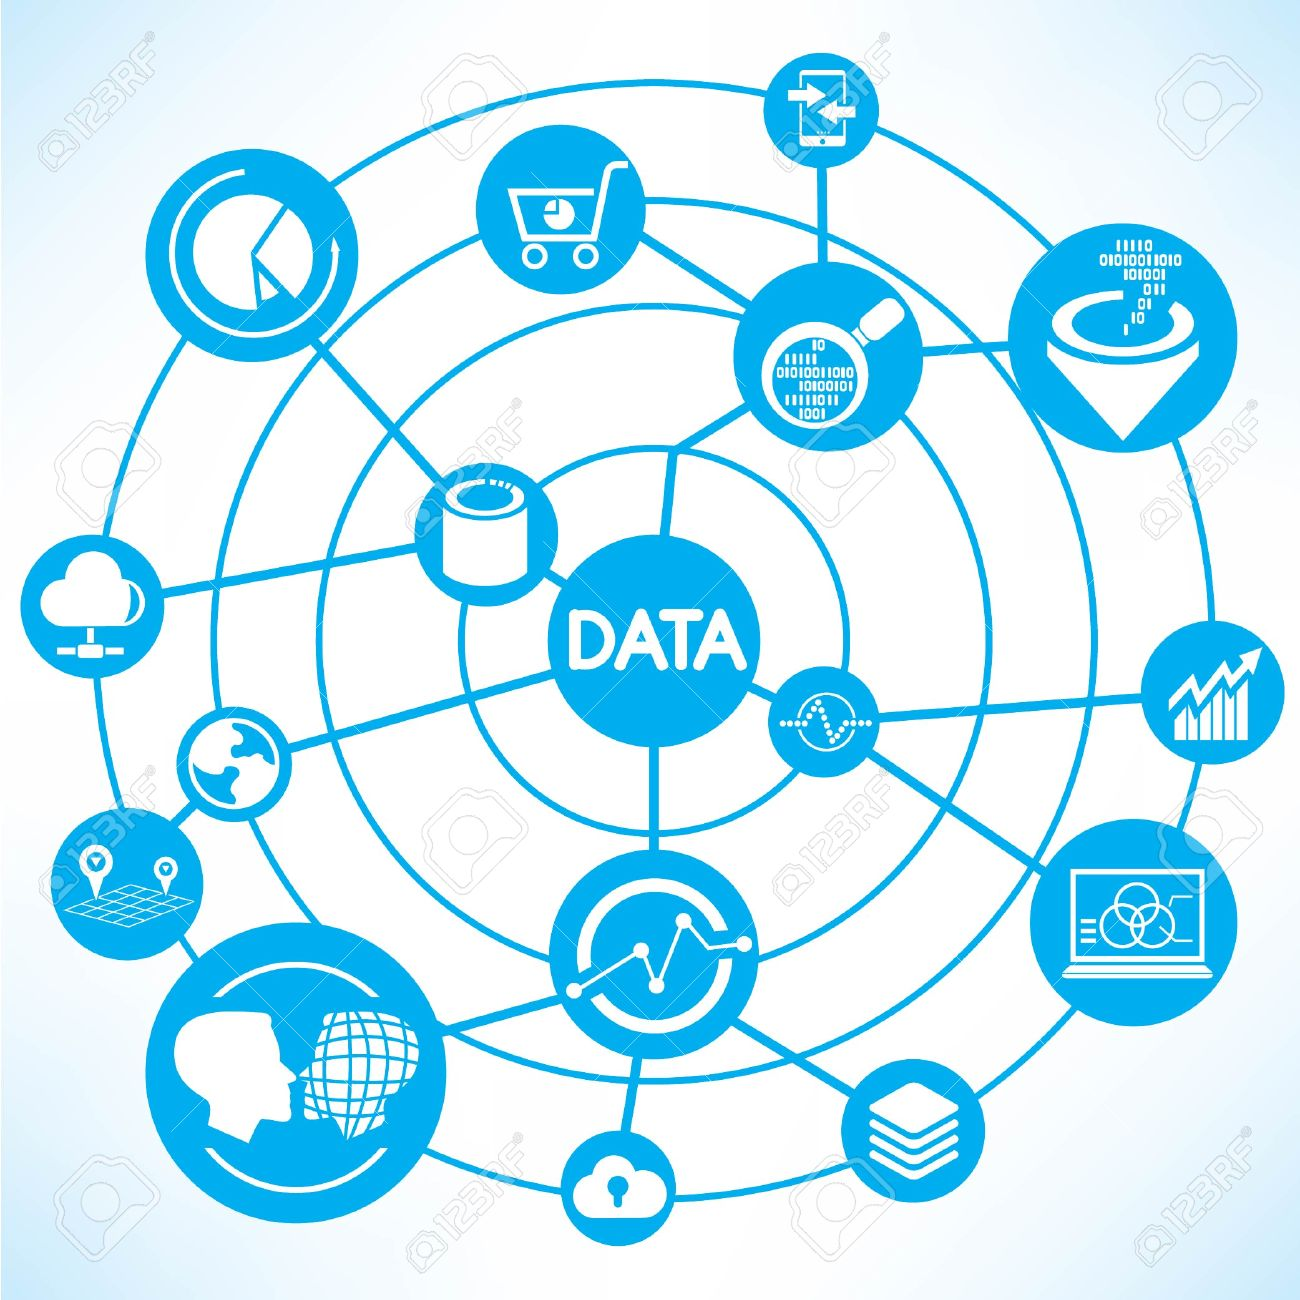
\includegraphics[width=0.3\textwidth]{Figures/internet-data.jpg}
    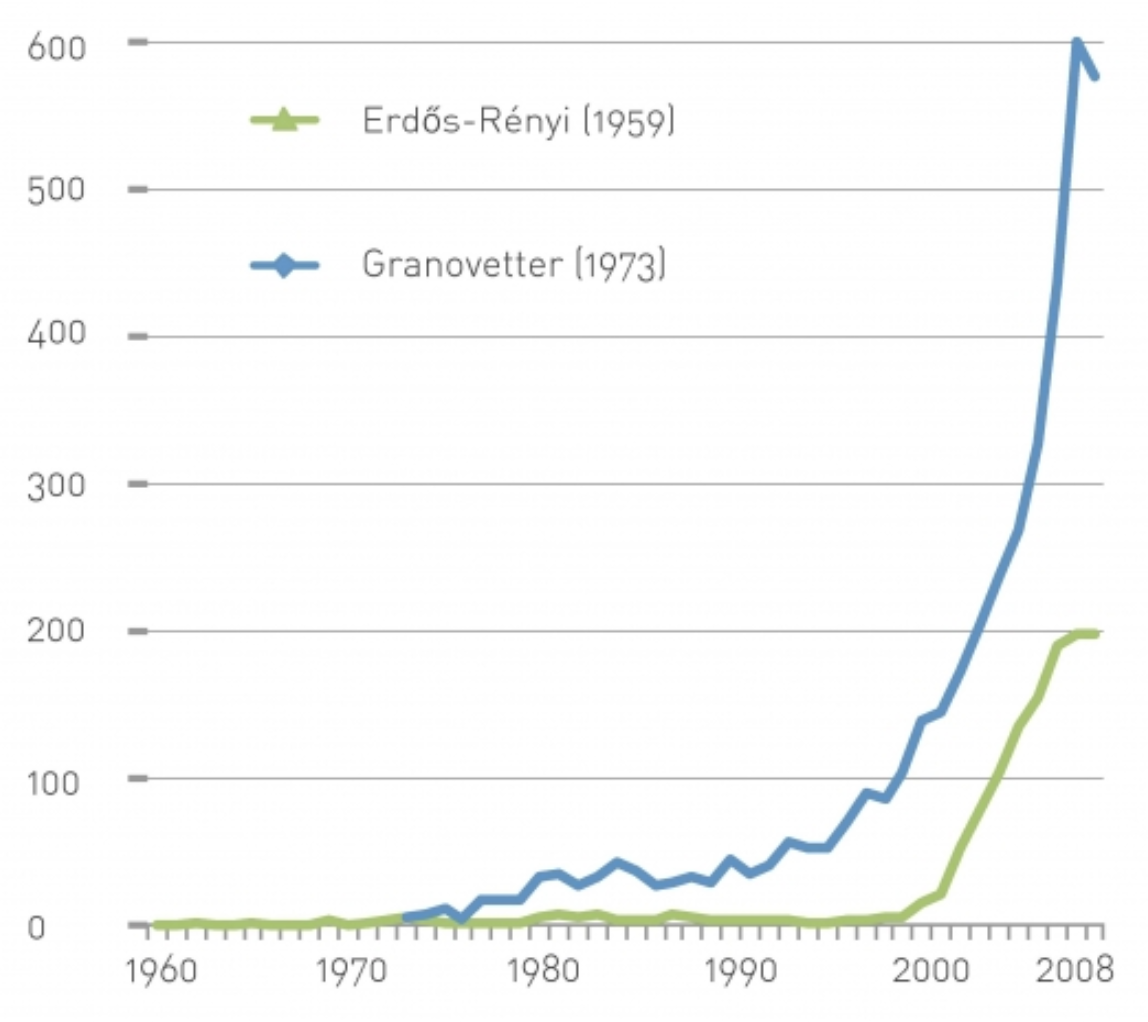
\includegraphics[width=0.3\textwidth]{Figures/ErdosRenyi-GranovetterCitations.png}
    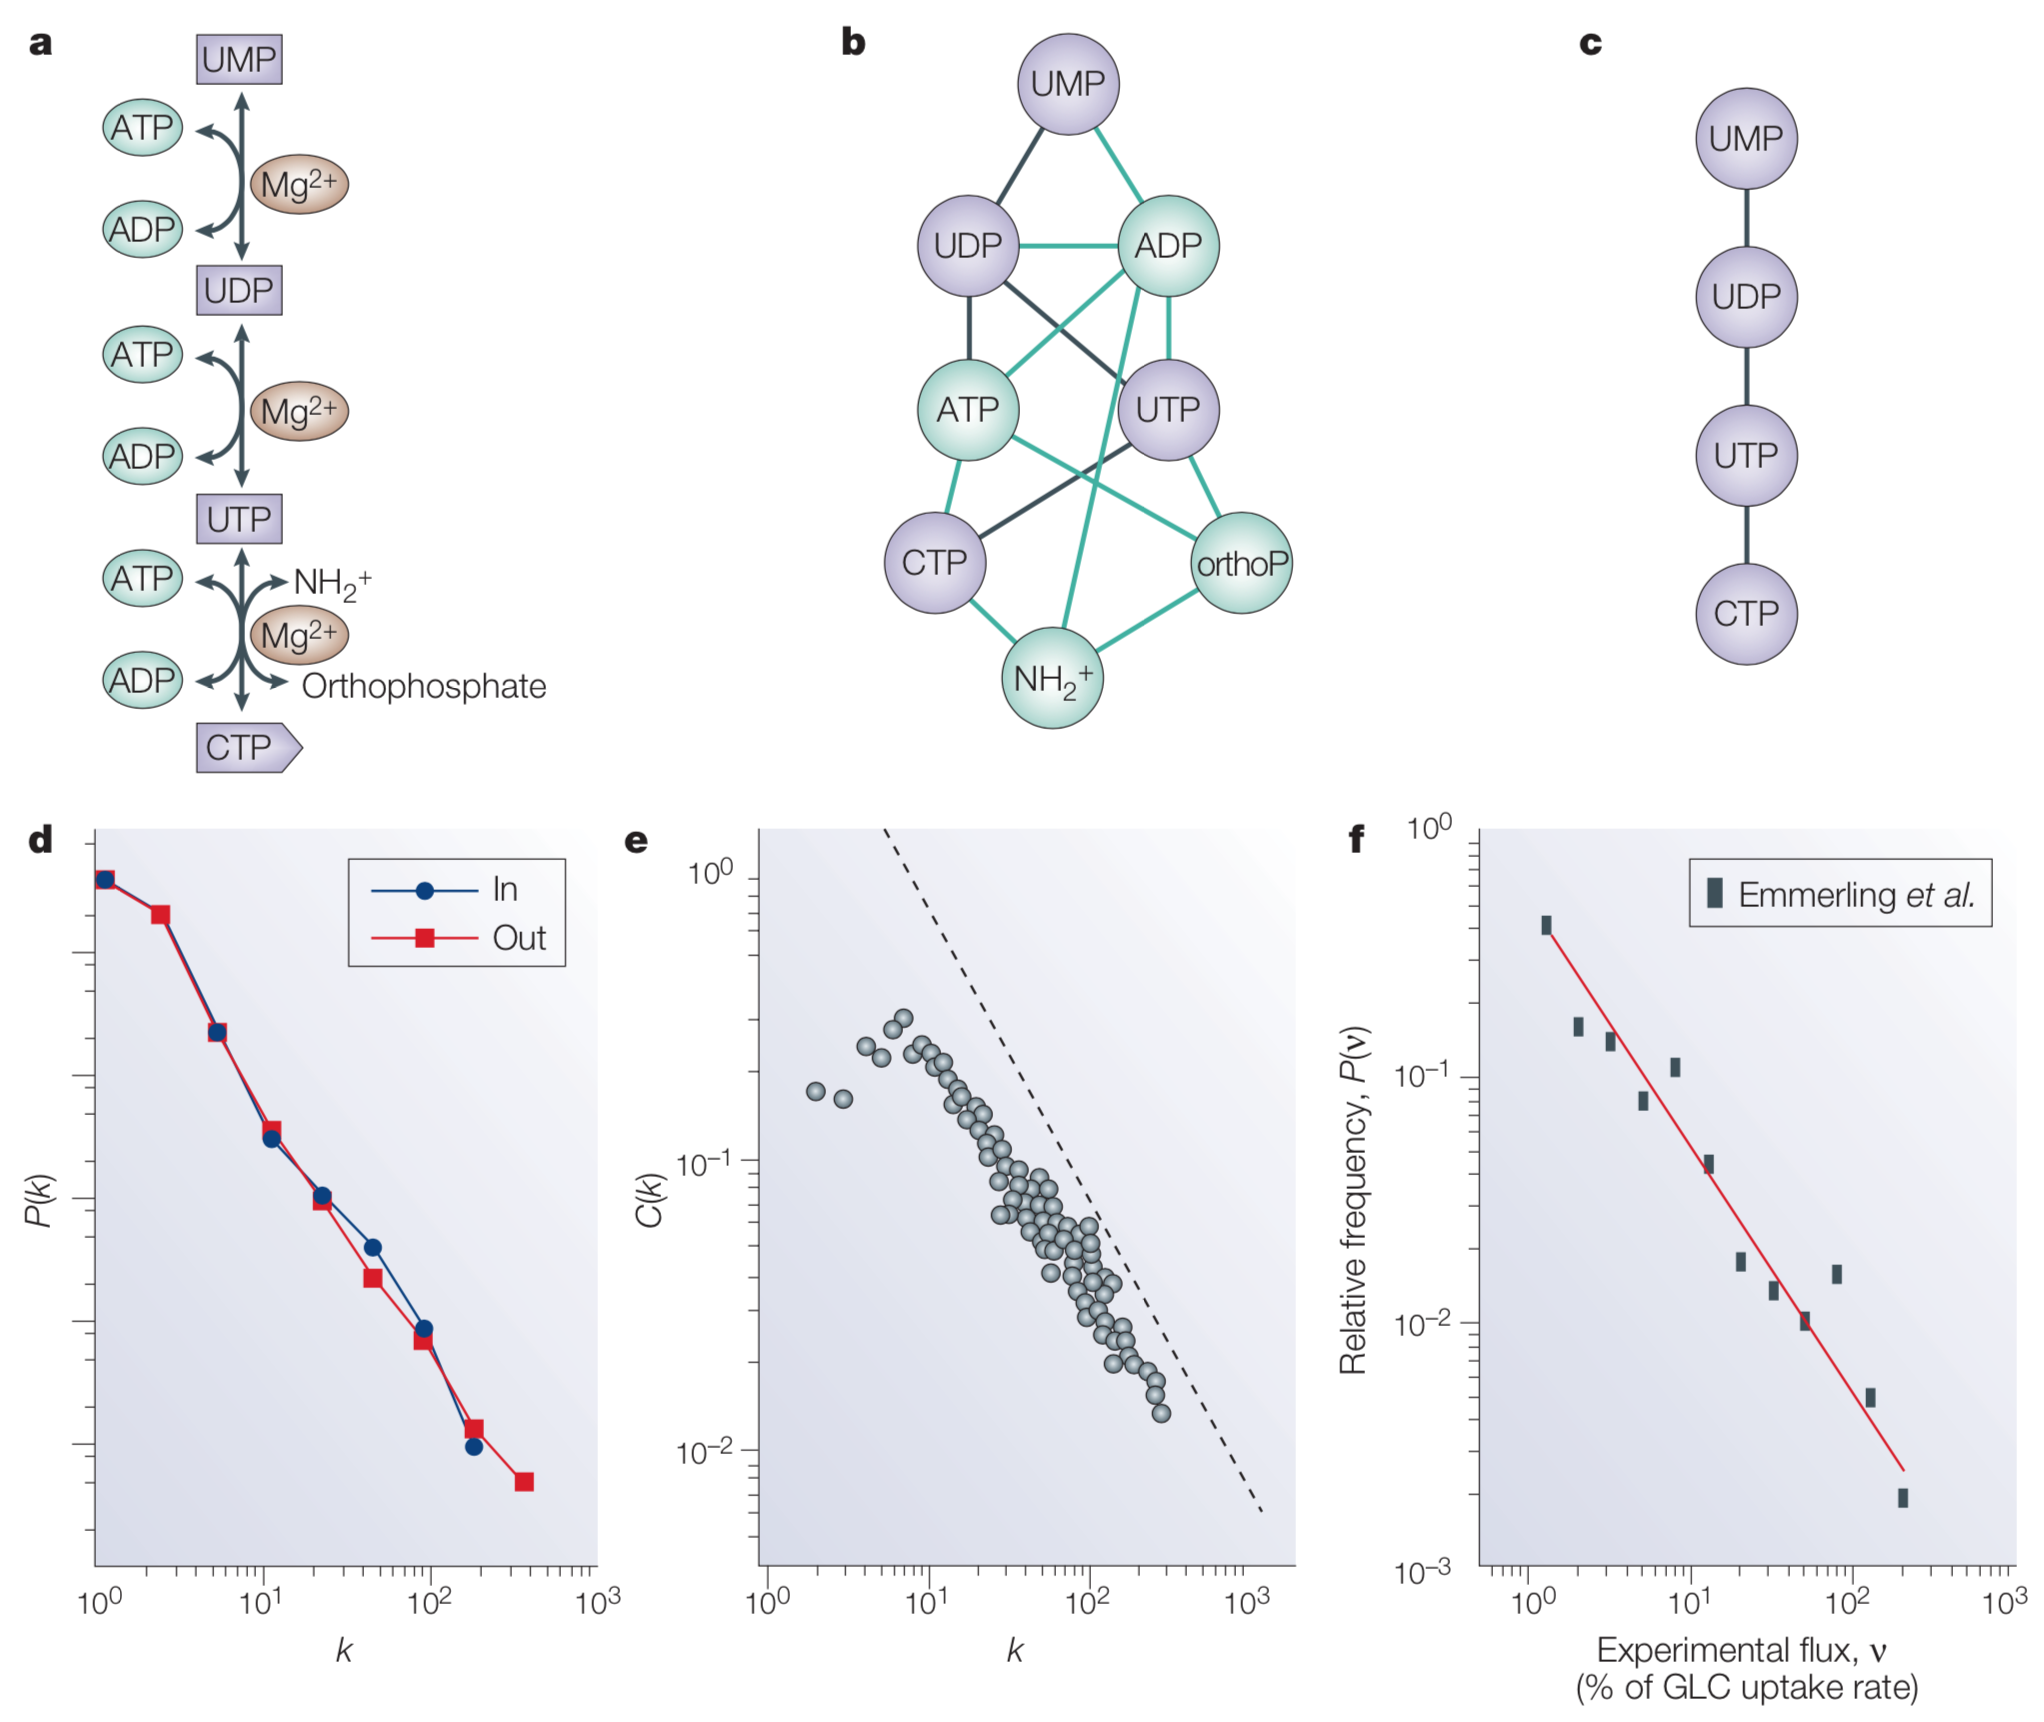
\includegraphics[width=0.4\textwidth]{Figures/NetworkCellBiologyIntro.png}
  \end{beamercolorbox}
  \vfill
\end{frame}
\note{In this frame point out that Erdos and Renyi were examining random graphs,
their properties, and related structures, but from a pure math perspective. They
knew there would be possible applications, but only mentioned that in passing.
While mathematicians worked on random graphs, sociologists were puzzling over
the small-world observation and the role that ``weak'' or distant social 
ties had on social influence. Also concurrently, biologists had been amassing
data on which proteins interact and how in cell biology. The advent of
the world wide web in the 1990s, where web pages were hosted on powerful and
plentiful Internet 
servers, and linked to other web pages, was both an important development of
a socio-techincal network, but also provided the infrastructure to host and
disseminate network data that would have been difficult to store, share, and
process were it not for advances in computing technology.}


% \begin{frame}{Outline}
%   \begin{enumerate}
%     \item My motivation for studying network science.
%     \item Historical \& mathematical development of network models.
%       \begin{itemize}
%         \item Focus on shortcomings of random graph models and how scale-free
%           network models solves them.
%       \end{itemize}
%     \item Networks in linguistic representations (CK).
%   \end{enumerate}
% \end{frame}
% \note{Why focus on scale-free network models? Because these are the most 
% parsimonious model (i.e.\ faithful, simple, and explanatory) of this wide variety 
% of observed behavior.}

% \begin{frame}{Personal motivation}
%   \begin{enumerate}
%     \item Understand the connection between social interaction networks and 
%       social clustering (consensus, ``bi-polarization'', or multiple clustering)
%       around knowledge, beliefs, opinions, attitudes etc. 
%     \item Understand the basis of network models of language and the evolution of language.
%     \item Build a critical knowledge base around networks to improve my work. 
%   \end{enumerate}
% \end{frame}

% \begin{frame}{French's model of the evolution of social power}
%   \centering
%   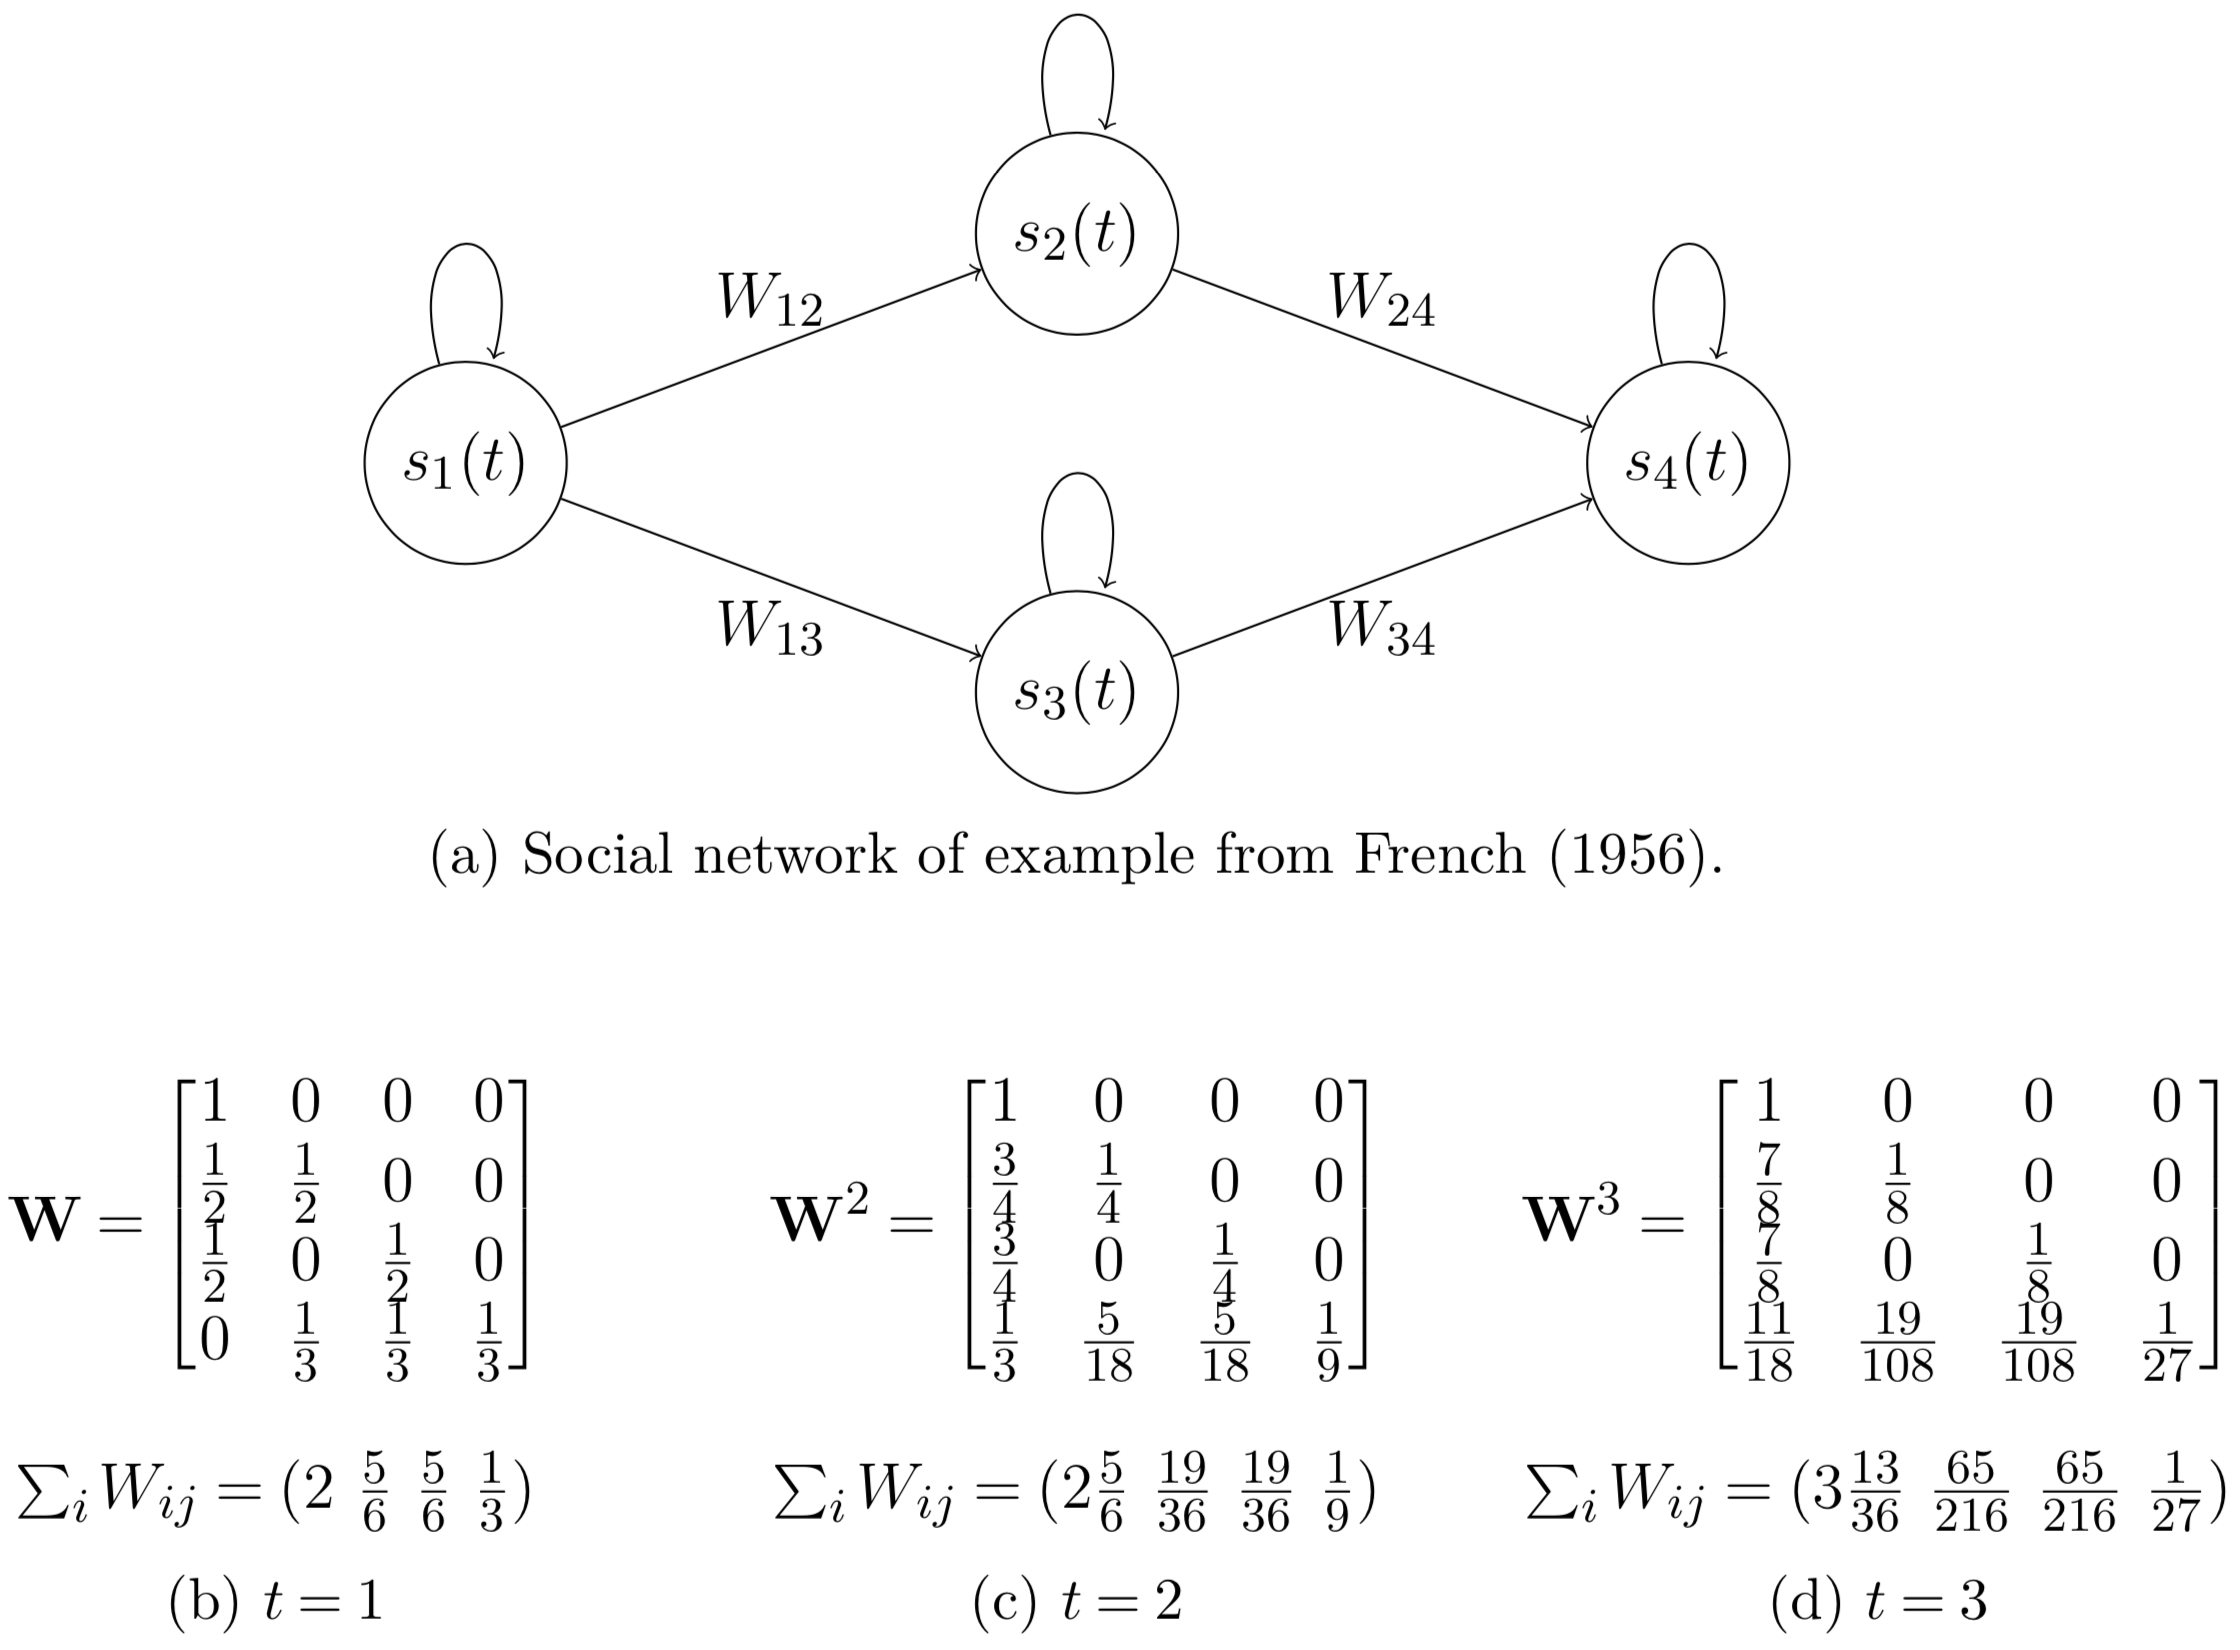
\includegraphics[width=0.8\textwidth]{Figures/FrenchPower.png}
% \end{frame}

% \begin{frame}{Granovetter's ``strength of weak ties''}
%   \begin{itemize}
%     \item In many cases, e.g.\ finding a job, it is not our closest
%       ``friends'', but casual or second-degree acquaintances who influence us.
%     \item Compare to Heider's social balance theory---weak ties have a
%       pre-assigned valence based on strong ties.
%   \end{itemize}
% \end{frame}

% \begin{frame}{Axelrod's model of ``The Dissemination of Culture''}
%   \begin{columns}[T]
%     \begin{column}{.48\textwidth}
%       Square lattice \\[1.5em]
%       \begin{tikzpicture} %[->,>=stealth',shorten >=2pt, line width=1pt, 
%         % node distance=2cm]  %, style ={minimum size=20mm}]
%       % \tikzstyle{every node}=[font=\huge]
%         \node [circle, draw] at (0, 0) (1) {}; % {$s_1(t)$};
%         \node [circle, draw] at (1, 0) (2) {}; % {$s_2(t)$};
%         \node [circle, draw] at (2, 0) (3) {}; % {$s_2(t)$};
%         \node [circle, draw] at (3, 0) (4) {}; % {$s_2(t)$};

%         \node [circle, draw] at (0, 1) (5) {}; % {$s_2(t)$};
%         \node [circle, draw] at (1, 1) (6) {}; % {$s_2(t)$};
%         \node [circle, draw] at (2, 1) (7) {}; % {$s_2(t)$};
%         \node [circle, draw] at (3, 1) (8) {}; % {$s_2(t)$};

%         \node [circle, draw] at (0, 2) (9) {}; % {$s_1(t)$};
%         \node [circle, draw] at (1, 2) (10) {}; % {$s_2(t)$};
%         \node [circle, draw] at (2, 2) (11) {}; % {$s_2(t)$};
%         \node [circle, draw] at (3, 2) (12) {}; % {$s_2(t)$};

%         \node [circle, draw] at (0, 3) (13) {}; % {$s_2(t)$};
%         \node [circle, draw] at (1, 3) (14) {}; % {$s_2(t)$};
%         \node [circle, draw] at (2, 3) (15) {}; % {$s_2(t)$};
%         \node [circle, draw] at (3, 3) (16) {}; % {$s_2(t)$};
%         % \path  (b) edge [loop above] (b);

%         % \node at (3, 1.75) {$W_{22}$};

%         % \draw[->] (a) to [bend left=20] node[above, bend left] {$W_{21}$} (b) ;
%         % \draw[->] (b) to [bend left=20] node[below, bend left] {$W_{12}$} (a) ;
%         \draw[-] (1) to (2); \draw[-] (2) to (3); \draw[-] (3) to (4);
%         \draw[-] (5) to (6); \draw[-] (6) to (7); \draw[-] (7) to (8);
%         \draw[-] (9) to (10); \draw[-] (10) to (11); \draw[-] (11) to (12);
%         \draw[-] (13) to (14); \draw[-] (14) to (15); \draw[-] (15) to (16);

%         \draw[-] (1) to (5); \draw[-] (2) to (6); \draw[-] (3) to (7); \draw[-] (4) to (8);
%         \draw[-] (5) to (9); \draw[-] (6) to (10); \draw[-] (7) to (11); \draw[-] (8) to (12);
%         \draw[-] (9) to (13); \draw[-] (10) to (14); \draw[-] (11) to (15); \draw[-] (12) to (16);
%       \end{tikzpicture}
%     \end{column}
%     \hfill
%     \begin{column}{.48\textwidth}
%       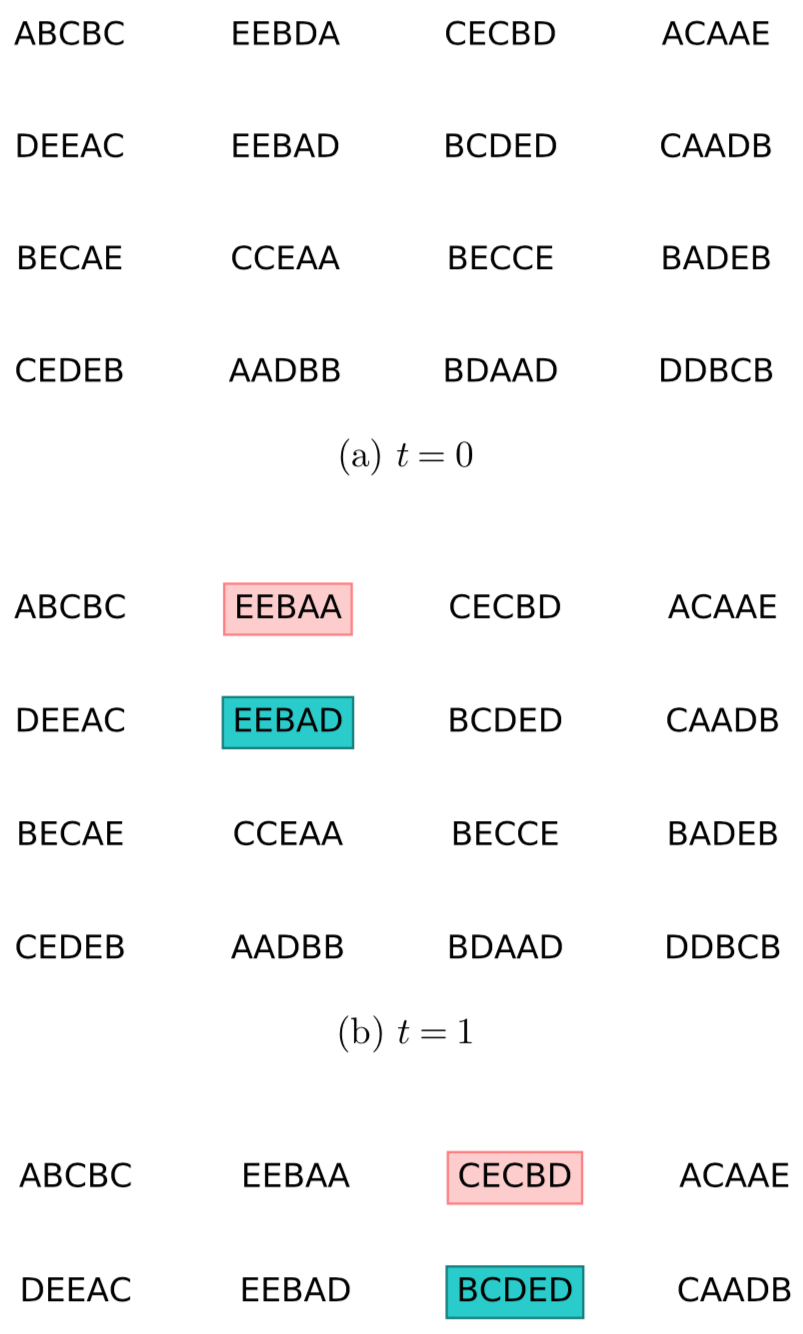
\includegraphics[width=0.8\textwidth]{Figures/AxelrodExample.png}
%     \end{column}
%   \end{columns}
% \end{frame}
% \note{Assumes agents are connected via a square lattice; \emph{homophily} implemented
% as increased likelihood to interact with similar others.}

% \begin{frame}{Axelrod on small-world and scale-free networks}
%   Klemm, et al., (2003)
% \end{frame}

\section{Development of scale-free networks}
\begin{frame}[plain]
  \vfill
  \centering
  \begin{beamercolorbox}[sep=8pt,center,shadow=true,rounded=true]{title}
    \usebeamerfont{title}\insertsectionhead\par%
    \color{oxfordblue}\noindent\rule{10cm}{1pt} \\[1em]

    \centering
    \begin{flushleft}
      Small \& Regular \\
        $\rightarrow$ Random \\
        $\rightarrow$ Watts-Strogatz small-world \\
        $\rightarrow$ Barabási-Albert scale-free
    \end{flushleft}
  \end{beamercolorbox}
\end{frame}

\begin{frame}{Overview}
  After some basics, I introduce random networks and their shortcomings. \\[.2em]

  Random network models fail to capture real-world...
  \begin{enumerate}
    \item Connectivity---random networks are not connected for the same average
      number of neighbors per node,
    \item Clustering---not enough neighbors of one node are neighbors of each other), or
    \item Degree distribution---too unlikely to find ``hubs'', or agents with orders
      of magnitude more neighbors than the average number of neighbors.
  \end{enumerate} 
  \vspace{.2em}
  
  Random networks do capture the small-world property of real-world networks.
\end{frame}

\begin{frame}{Graph and network basics}
  $N$: number of nodes \\
  $L$: number of links \\
  $k_i$: ``degree'' of node $i$ (number of network neighbors) \\[1em]

  Indicate average/expectation using angle brackets
  \begin{center}
    \begin{itemize}
      \item $\langle k \rangle = \frac{1}{N} \sum_{i=1}^N k_i$
      \item $L = \frac{1}{2} \sum_{i=1}^N k_i$, where $1/2$ corrects for double counting 
    \end{itemize}

  \end{center}
\end{frame}

\begin{frame}{Network or ``graph''?}
  Network refers to a real-world entity or a model of a real-world entity. 
  Graph refers to a purely abstract mathematical entity. \\[2em]

  \centering
  \begin{tabular}{cc}
    \textbf{Network} & \textbf{Graph} \\
    \hline
    Node & Vertex \\
    Link & Edge 
  \end{tabular}
\end{frame}

\begin{frame}{Degree distribution}
  Call the histogram of degree counts $N_k$, indicating the number of nodes
  with degree $k$. \\[1em]

  Then the degree distribution is
  \[ p_k = N_k / N \]

  We can now treat $k_i \sim p_k$ as a random variable and its expectation is
  \[ \langle k \rangle = \sum_{k=0}^\infty k p_k \]

  $p_k$ encodes network structure and predicts behavior
\end{frame}



\begin{frame}{Path lengths}
  Path is a tuple of steps over links from node $i$ to node $j$. 
  $d_{ij}$ is the ``distance'', the minimum-step path from $i$ to $j$. \\[1em]
  $d_\text{max} = \max_{ij} d_{ij}$ is the ``diameter'' of the network.  \\[1em]

  Average path length:
  \[ \langle d \rangle = \frac{1}{N(N-1)} \sum_{\substack{i=1,\ldots,N \\ j < i}} d_{ij} \]
  
  $d_{ij}$ found via breadth-first search algorithm.
\end{frame}

\begin{frame}{$d_{ij}$ via breadth-first search}
  \centering
  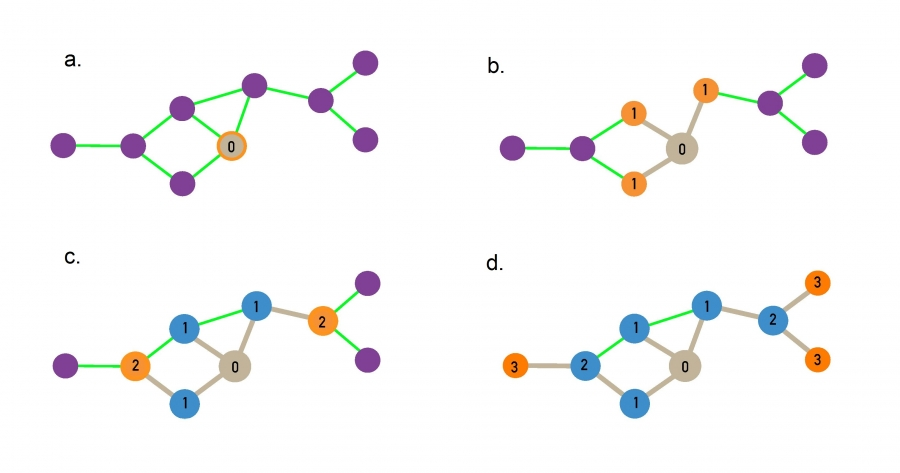
\includegraphics[width=0.75\textwidth]{Figures/bfs.jpg} \\
  % \hline
  A certain form of breadth-first search is used for computing 
  $\langle d \rangle$ even on the largest of networks such as Facebook
  (see \url{https://arxiv.org/abs/1111.4503v1} and 
  \url{https://arxiv.org/abs/1111.4570} that show $\langle d \rangle \approx 4$
  on Facebook.
\end{frame}

\begin{frame}{Clustering coefficient}
  If node $i$ has degree $k_i$, then local clustering coefficient is
  the number of existing links between neighbors, $L_i$ divided by 
  the number of possible links between neighbors, ${k \choose 2}$:

  \[ C_i = \frac{2 L_i}{k_i(k_i - 1)} \]
\end{frame}
\note{Here can explain the binomial factor that will appear many times. 
${n \choose 2}$. Could also draw an example if that would be useful.
See notes for that example.}

% \begin{frame}{Global clustering coefficient}
%   Number of triangles divided by the number of possible triangles. \\[1em]

%   \[ 
%     C_{\triangle} = 
%       \frac{3 \cdot \text{\#triangles (closed triples)}}{\text{\#connected triples}} 
%   \]

%   Also called the ``ratio of transitive triplets'', where a transitive
%   triplet are three nodes such that if $x,y$ are connected, and $y,z$ 
%   are connected, then $x,z$ are connected.
% \end{frame}
% \note{See example in notebook.}

\section{Random graphs}
\begin{frame}[plain]
  \vfill
  \centering
  \begin{beamercolorbox}[sep=8pt,center,shadow=true,rounded=true]{title}
    \usebeamerfont{title}\insertsectionhead\par%
    \color{oxfordblue}\noindent\rule{10cm}{1pt} \\[1em]

    \centering
    Our starting point for developing scale-free networks

  \end{beamercolorbox}
\end{frame}

\begin{frame}{Construction of random networks}
  \underline{Init:} $N$ isolated nodes; probability $p$ two nodes are linked.

  \underline{Procedure:} 
  \begin{itemize}
    \item Iterate through all ${N \choose 2}$ pairs of nodes. For each node,
      \begin{itemize}
        \item Draw $x \sim \text{Uniform}$. 
        \item If $x < p$ add link between nodes in pair. 
      \end{itemize}
  \end{itemize}
\end{frame}

\begin{frame}{Link distribution of random networks}
  What is the probability that $L$ links are added, $p_L$? \\[1em]
  \begin{itemize}
    \item ${N \choose 2}$ possible links with $L$ actual links, there are
      ${\frac{N(N-1)}{2} \choose L}$ ways to do that.
    \item Probability $L$ edges are added: $p^L$.
    \item Probability that $\frac{N(N-1)}{2} - L$ edges are not added:
      $p^{\frac{N(N-1)}{2} - L}$.
  \end{itemize}
  Put these all together to get
  \[ p_L = {\frac{N(N-1)}{2} \choose L} p^L p^{\frac{N(N-1)}{2} - L} \]
\end{frame}

\begin{frame}{Degree distribution of random networks}
  \begin{itemize}
    \item Number of ways to choose the $k$ links that are present:
      ${N-1 \choose k}$.
    \item Probability $k$ links at a node is $p^k$.
    \item Probability $N-1-k$ links are not present at that node: $p^{N-1-k}$.
  \end{itemize}
  Again this leads to a binomial distribution
  \[
    p_k = {N-1 \choose k} p^k (1-p)^{N-1-k}
  \]
\end{frame}

\begin{frame}{Poisson approximates random degree distribution}
  \[
    p_k = {N-1 \choose k} p^k (1-p)^{N-1-k}
  \]

  But often $\langle k \rangle \ll N$, which means that $p_k$ can be 
  approximated by a Poisson distribution, which simplifies calculations:

  \[
    p_k = e^{-\langle k \rangle} \frac{\langle k \rangle^k}{k!}
  \]

  With Poisson, e.g., we know that $\sigma_k = \langle k \rangle^{\frac{1}{2}}$.
\end{frame}

\begin{frame}{Random distributions underestimate $k_{max}$}
  To see how, we perform the following calculation. Sociologists calculate
  that in the real-world, $\langle k \rangle \approx 1000$. $N \approx 7 \cdot 10^9$.

  The maximum $k$ occurs for
  just one of the $N$ nodes, so $1 - P(k_{max}) \approx 1/N$. \\[.25em]

  \begin{columns}
    \begin{column}{.48\textwidth}
      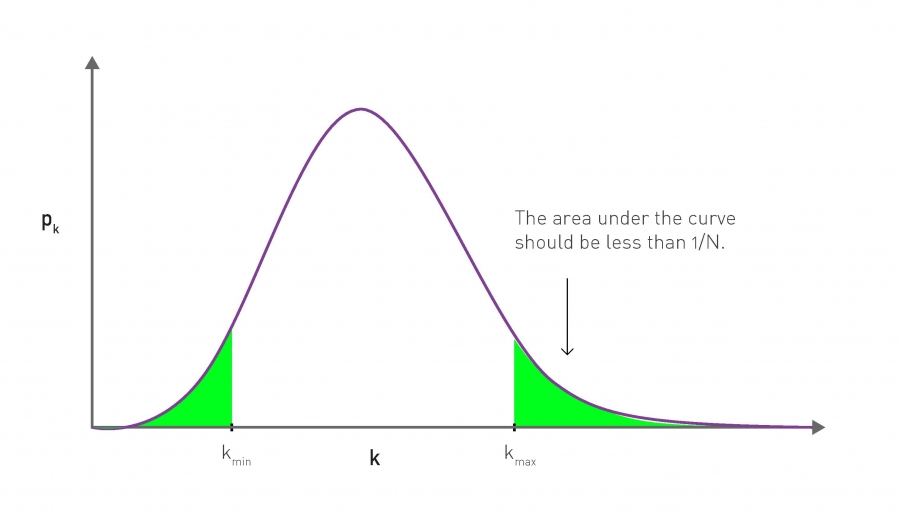
\includegraphics[width=\textwidth]{Figures/maxDegreeCalc.jpg}
    \end{column}
    \begin{column}{.48\textwidth}
      \begin{align*}
        1 - P(k_{\max}) & = 1 - e^{-\langle k \rangle} \sum_{k=0}^{k_{\max}} 
                                                     \frac{\langle k \rangle^k}{k!}  \\
                        & = e^{-\langle k \rangle} \sum_{k=k_{\max}+1}^{\infty} 
                                                     \frac{\langle k \rangle^k}{k!}  \\
                        & \approx e^{-\langle k \rangle} \frac{\langle k \rangle^{k_{\max}+1}}{(k_{\max} + 1)!}
      \end{align*}
    \end{column}
  \end{columns}
  Setting this equal to $1/N$ and solving via magic yields $k_{max} = 1,185$.
\end{frame}
\note{But some people know many thousands of others personally. Random networks
\emph{are not scale-free}---the $k!$ term in denominator eliminates large-$k$
nodes.}
\begin{frame}{Random degree distributions don't match observation}
  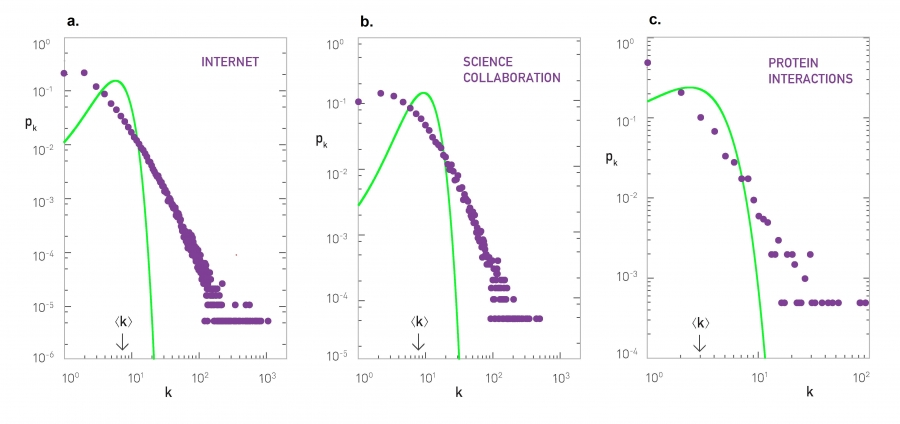
\includegraphics[width=1.1\textwidth]{Figures/poissonVsRealDegDist.jpg}
\end{frame}

\begin{frame}{Random network connectedness regimes}
  As $p$ increases, random networks go from essentially disconnected, to the
  emergence of a large connected component (the ``giant component''), to
  being totally connected when $p > \frac{\ln N}{N}$. \\[.25em]

  Connected also implies $\langle k \rangle > \ln N$. 

  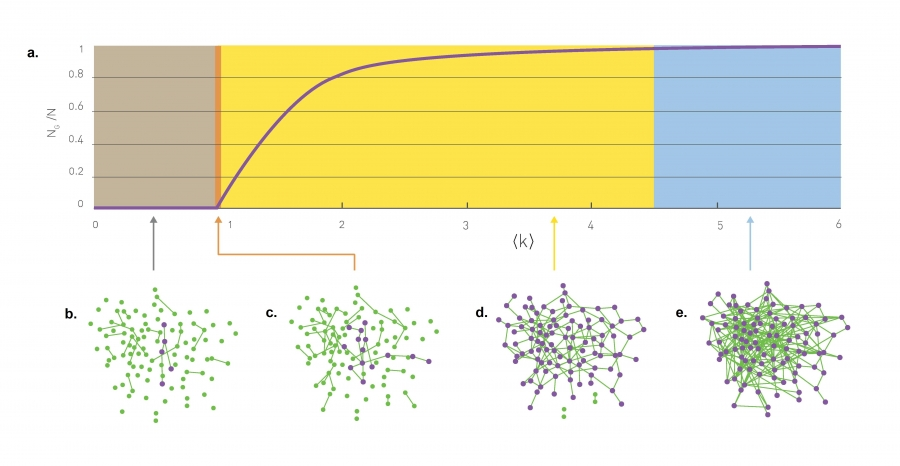
\includegraphics[width=\textwidth]{Figures/randomRegimes.jpg}
\end{frame}


\begin{frame}{Random network connectedness regimes}
  \centering
  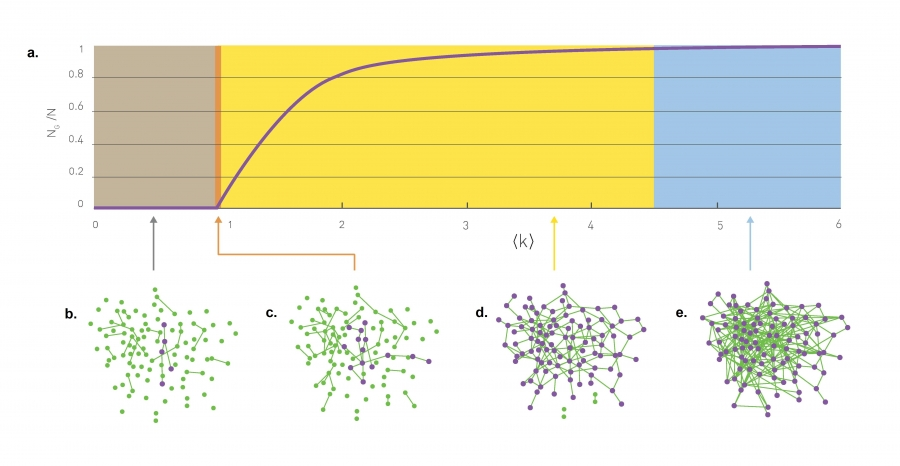
\includegraphics[width=.6\textwidth]{Figures/randomRegimes.jpg} \\
  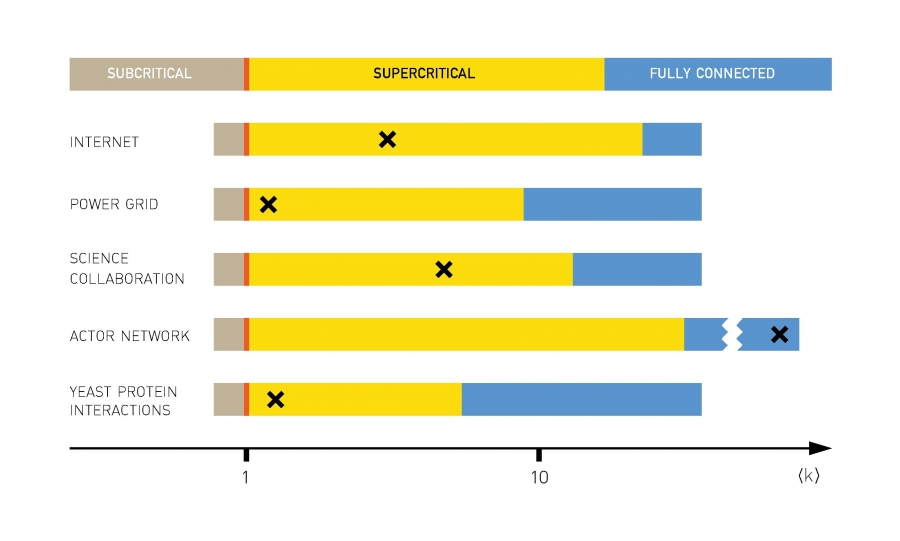
\includegraphics[width=.7\textwidth]{Figures/randomRegimeCompareRealworld.jpg}
\end{frame}
\note{Takeaway here is that random network theory predicts these connected
real-world networks would not be connected based on $\langle k \rangle$.}


\begin{frame}{Random network clustering coefficient}
  Random network theory predicts a $1/N$ dependence (green line in figures)
  and no $k$-dependence.
  \begin{columns}
    \begin{column}{.48\textwidth}
      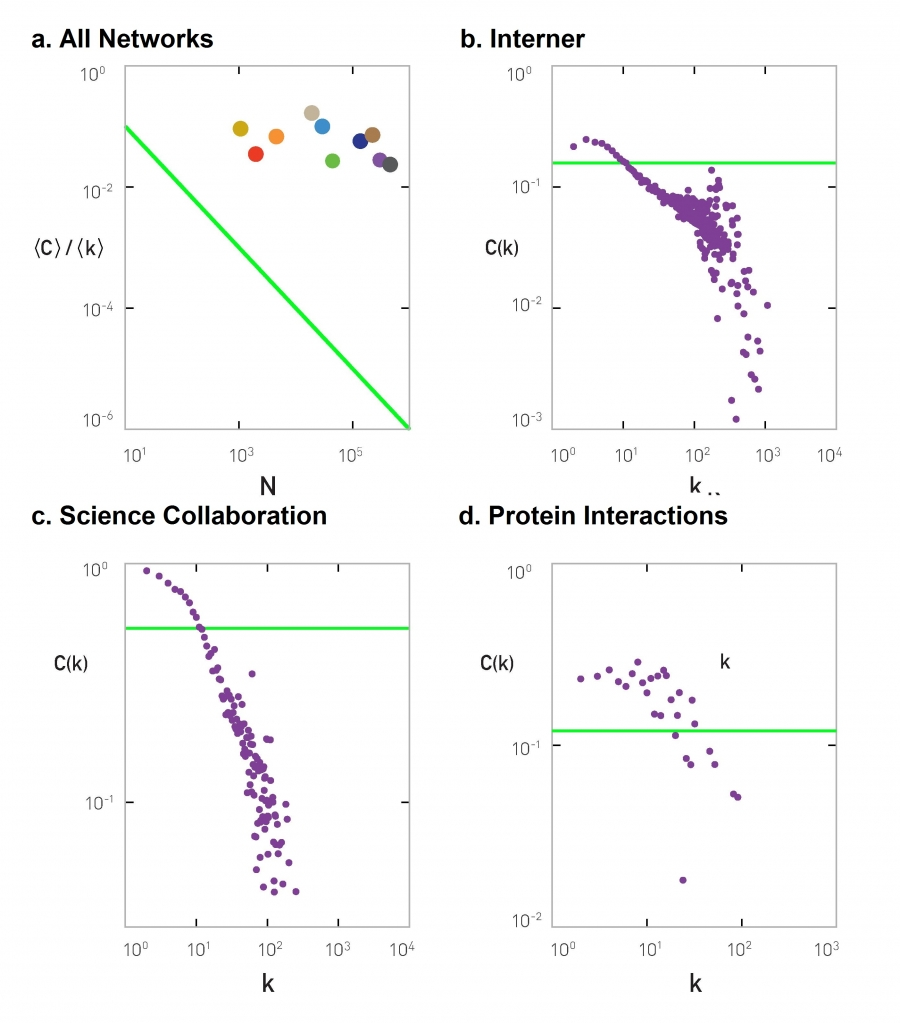
\includegraphics[width=\textwidth]{Figures/realNetworkClusteringNotRandom.jpg} 
    \end{column}
    \begin{column}{.48\textwidth}
      \small
      Recall \[ C_i = \frac{2 \langle L_i \rangle}{k_i(k_i-1)}, \] 
      \[ \langle L_i \rangle = p \frac{k_i(k_i - 1)}{2}. \]
      Then for large $N$, \[ C_i = p = \frac{\langle k \rangle}{N}. \] 
    \end{column}
  \end{columns}
\end{frame}

\begin{frame}{Random networks are small-world networks}
  \centering
  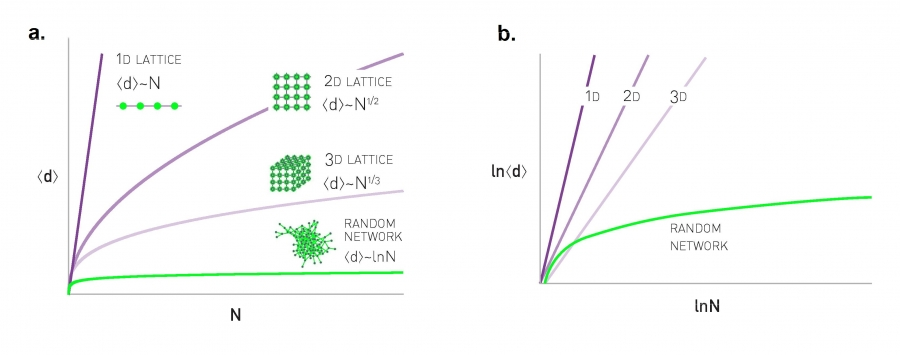
\includegraphics[width=1.1\textwidth]{Figures/randomSmallWorld.jpg} 
\end{frame}

\begin{frame}{Random networks are small-world networks}
  \centering
  Count number of nodes up to distance $d$:
  \[
    N(d) \approx 
      1 + \langle k \rangle + \langle k \rangle^d + \cdots + \langle k \rangle^d =
      \frac{\langle k \rangle^{d+1} - 1}{\langle k \rangle - 1}
  \]
  For large $N,~\langle k \rangle \gg 1$, $N(d_{\max}) \approx N$ and 
  $N(d) \approx \langle k \rangle^d$. Then 

  \[\langle k \rangle^{d_{\max}} \approx N\]
  which leads to the \emph{small-world condition}
  \[d_{\max} \approx \frac{\ln N}{\ln \langle k \rangle}\]
\end{frame}

\begin{frame}{Random networks are small-world networks}
  In $d_{\max} \approx \frac{\ln N}{\ln \langle k \rangle}$, this is often
  dominated by very few long paths, and so $\langle d \rangle \approx d_{\max}$,
  so the small-world condition is

  \[
    \langle d \rangle \lessapprox \frac{\ln N}{\ln \langle k \rangle}
  \]
  \centering
  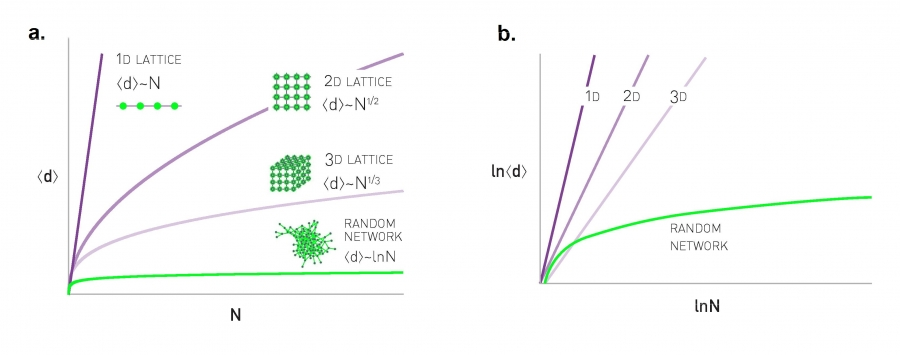
\includegraphics[width=0.8\textwidth]{Figures/randomSmallWorld.jpg} 
\end{frame}

\begin{frame}{Watts-Strogatz model: clustered small-world}
  \vspace{-1em}
  \centering
  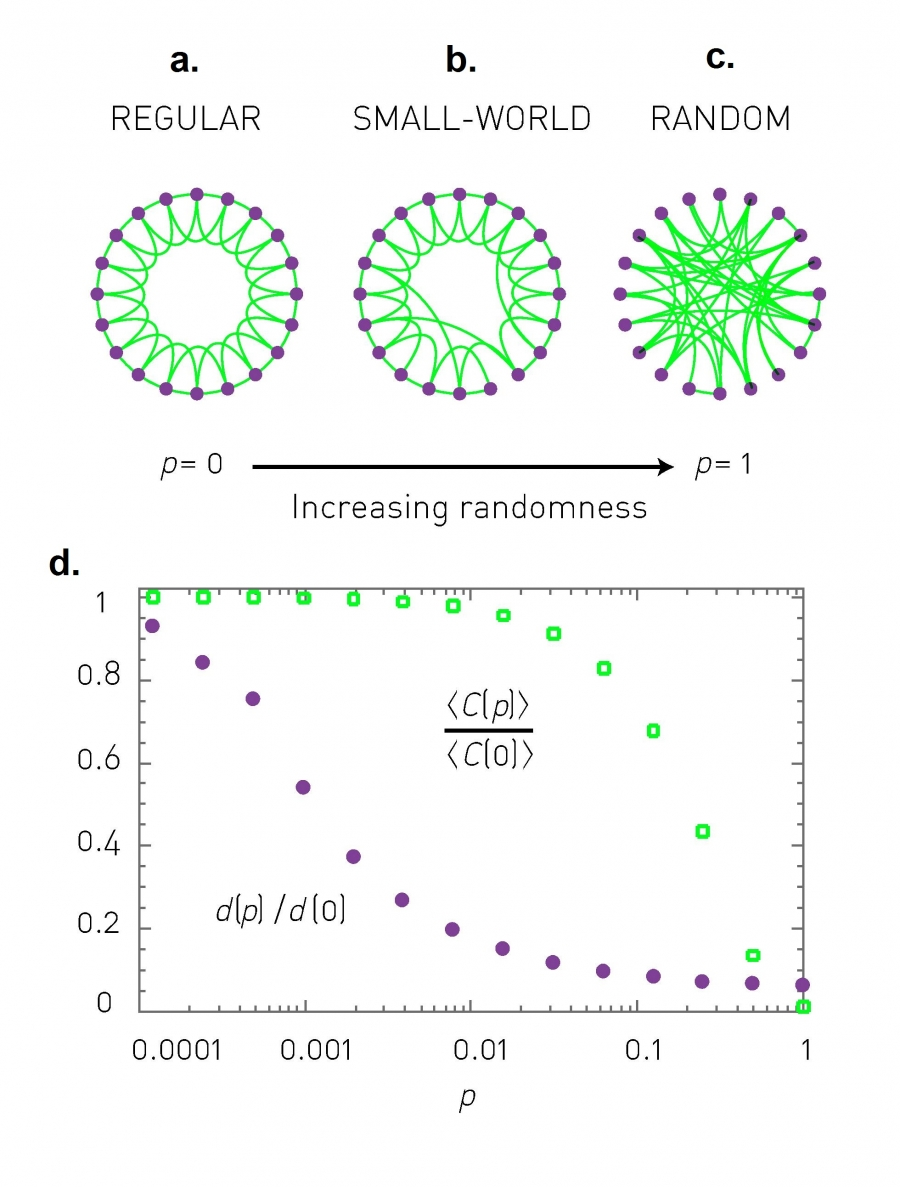
\includegraphics[width=0.6\textwidth]{Figures/wattsStrogatz.jpg}
\end{frame}

\begin{frame}{Meaning of ``scale-free''}
  We go to ``continuum formalism'' to make calculations easy. The $k^{th}$
  moment of $p_k$ is
  \[
    \langle k^n \rangle = \sum_{k_{\min}}^\infty k^n p_k = 
      \int_{k_{\min}}^\infty k^n p(k) dk
  \]
  The second moment is used to calculate variance, 
  $\sigma_k^2 = \langle k^2 \rangle - \langle k \rangle^2$.
  \vspace{.5em}
  The power-law degree distribution is $p(k) = Ck^{-\gamma}$. Then
  \[
    \langle k^n \rangle = C \int_{k_{\min}}^\infty k^n k^{-\gamma} dk 
                        = C \Bigl[ k^{n - \gamma + 1} \Bigr|_{k_{\min}}^\infty
  \]
\end{frame}

\begin{frame}{Meaning of ``scale-free''}
  \[
    \langle k^n \rangle = C \int_{k_{\min}}^\infty k^n k^{-\gamma} dk 
                        = C \Bigl[ k^{n - \gamma + 1} \Bigr|_{k_{\min}}^\infty
  \]
  To finish evaluating this integral, we need to find the limit of the 
  first term as $k \to \infty$. When is this finite? When
  \[
    n - \gamma + 1 \le 0,
  \]
  or,
  \[
    \gamma \ge n + 1
  \]
  So if $2 \le \gamma < 3$, then $\langle k^2 \rangle, \sigma_k \to \infty$,
  making hubs (large $k$ nodes) much more likely.
\end{frame}

\begin{frame}{Large $\sigma_k$ in real-world networks}
  \vspace{-1em}
  \centering
  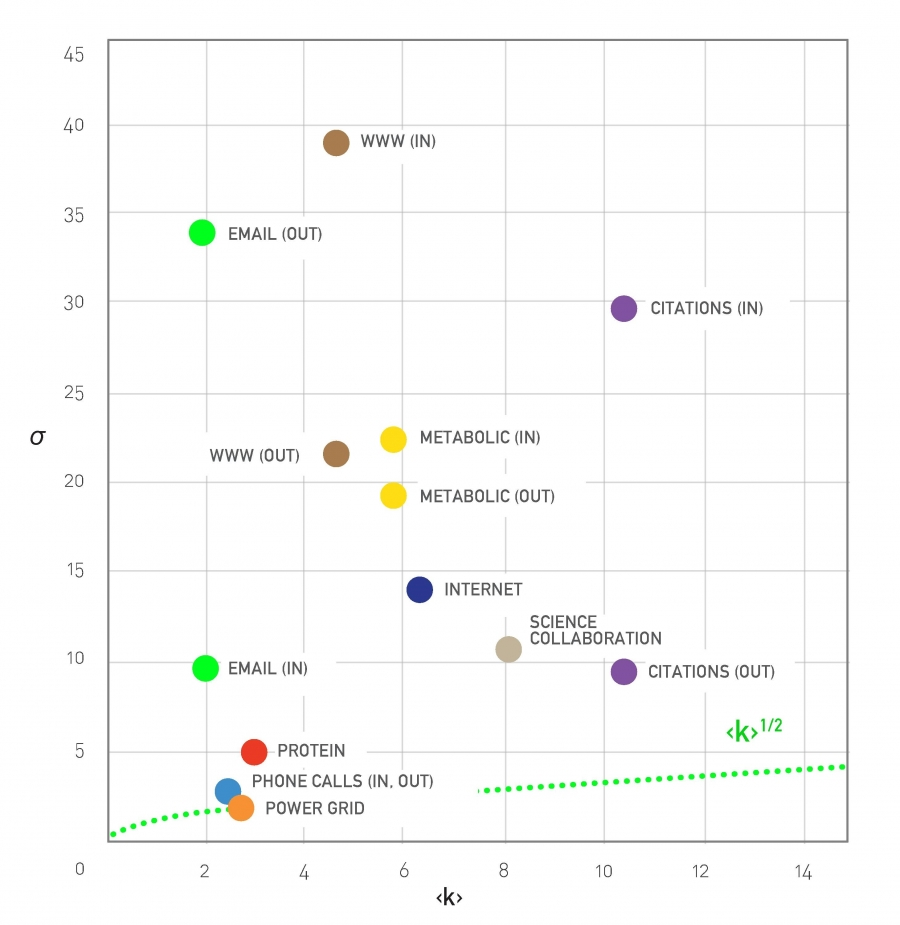
\includegraphics[width=0.7\textwidth]{Figures/largeStddevRealNetworks.jpg}
\end{frame}

\begin{frame}{Poisson vs. Scale-free}
  \vspace{-1em}
  \centering
  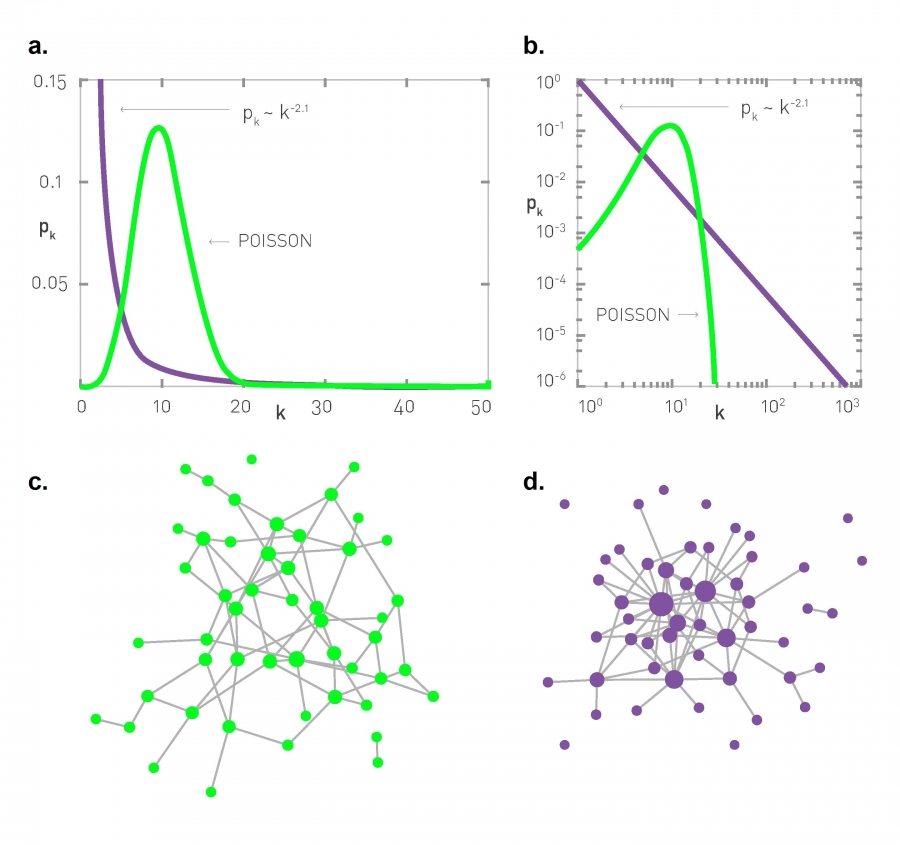
\includegraphics[width=0.75\textwidth]{Figures/poissonVsScalefree.jpg}
\end{frame}


\begin{frame}{$\langle d \rangle$ regimes for scale-free networks}
  \vspace{-1em}
  \centering
  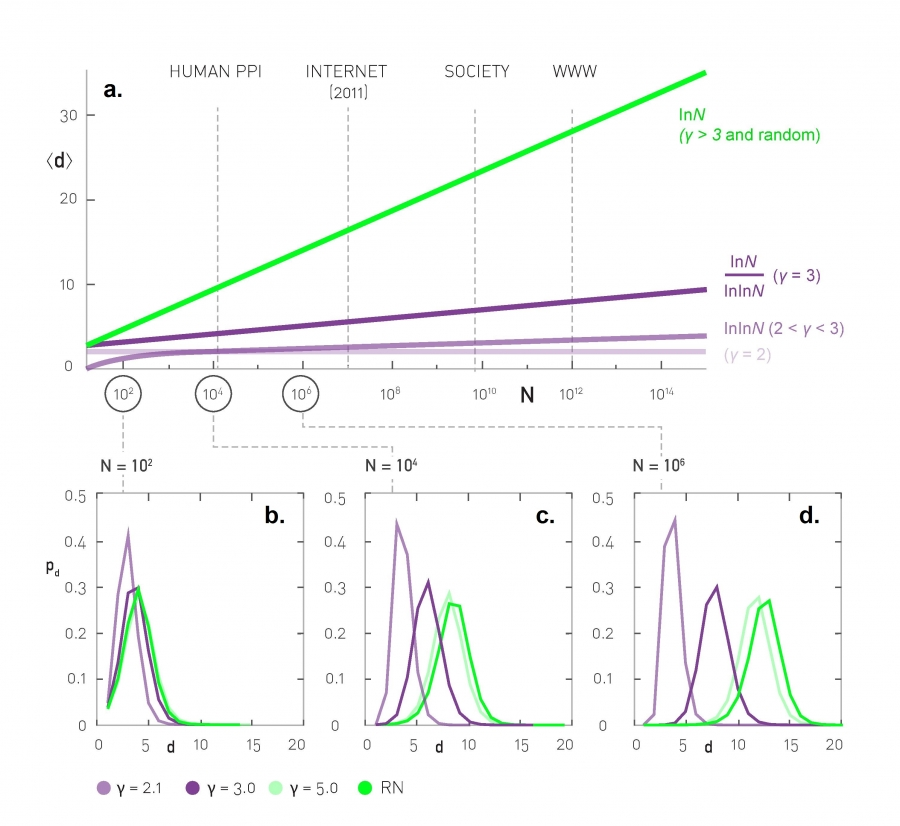
\includegraphics[width=0.8\textwidth]{Figures/scaleFreeDistances.jpg}
\end{frame}

\begin{frame}{Other $\gamma$-dependent properties}
  \vspace{-1em}
  \centering
  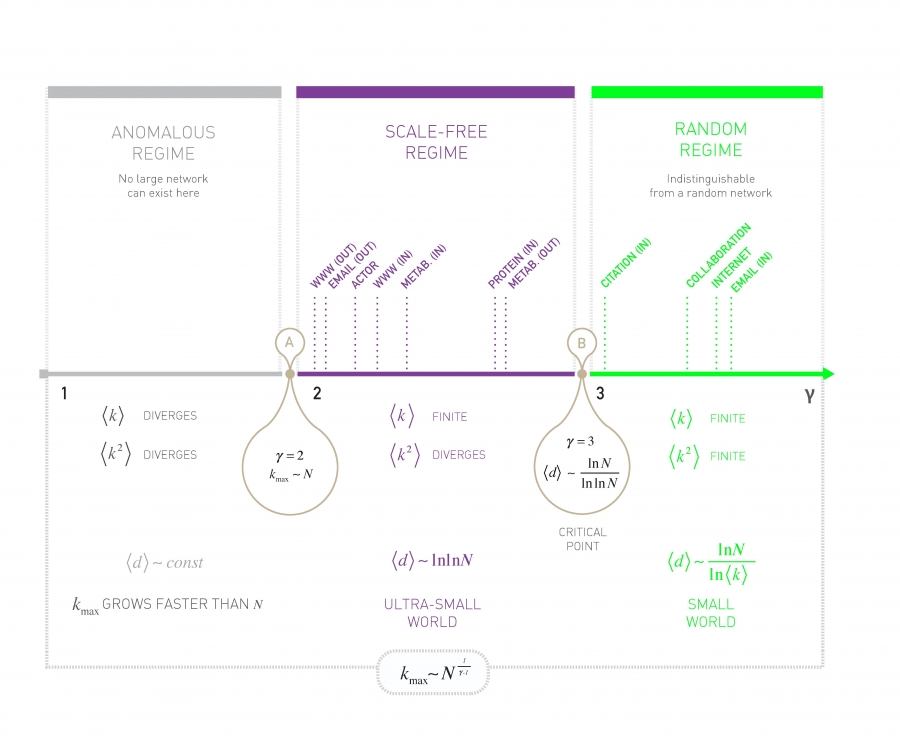
\includegraphics[width=0.9\textwidth]{Figures/gammaDependentPropBox.jpg}
\end{frame}

\end{document}
